\chapter{行波管的放大能力} \label{ch4}
行波管是一种放大微波信号的器件,因此放大能力是它的主要参数,并且通常用增益来表示。增益($ G $)的意义如下:
\begin{equation} \label{eq:ch4-1}
	G=10\lg\frac{P_\text{出}}{P_\text{入}}(\textrm{dB})
\end{equation}
其中$ P_\textrm{入} $为加到行波管输入端待放大信号的功率,而$ P_\text{出} $是在输出端得到的放大后的信号功率。$ G $的单位是分贝,$ G=10 $分贝相当于放大十倍;20分贝相当于放大100倍;30分贝相当于放大1000倍等等。

微波信号在行波管内所以能被放大,是因为在螺旋线内流动的电子注与外加信号所建立的高频场发生了能量转换的结果。因而行波管放大能力将主要由这两方面的条件及相互作用情况所决定。本章先着重定性讨论这些因素对行波管增益的影响,最后简略介绍一下增益计算的主要问题。
\section{电子注参量对增益的影响}
中小功率行波管中采用的电子注,基本上都是圆形截面的实心电子注。可以用三个参量来表征这种电子注的主要状况即:电子注电流$ I_0 $、电子速度$ v_e $(它是螺旋线电压$ U_0 $所决定)以及电子注截面半径$ b $。下面分别看看这三个因素改变时行波管增益如何随之变化。
\subsection{电子注电流的影响}	
	电子注电流($ I_0 $)越大,则参与同高频场相互作用的电子数目就相应增多。这就是说,有较多的电子受高频场的作用而群聚在减速场里,从而也就有更多的电子将其一部分动能转换为高频场的能量,使信号得到更充分的放大。所以电子注电流$ I_0 $增加对提高增益有利。
\subsection{电子注电压的影响}	
	电压$ U_0 $越高,则电子速度越快,惯性越大,因而在高频场作用下,就比较不容易改变其速度和位置,即不易很快地群聚起来。要使电子迅速群聚起来,就要有较强的高频电场,即需要在行波管输入端送进较强的信号功率($ P_\text{入} $)。否则,因电子注群聚较慢,输出端得到的放大后的信号功率就会减小。由\ref{eq:ch4-1}式可以看出,无论是输入功率$ P_\text{入} $增加,还是输出功率$ P_\text{出} $减小,都直接导致行波管的增益下降。所以,在同样的电子注功率(即:乘积$ U_0I_0 $)下,通常是较大的电流及较低的电压对提高管子增益有利些。	
	
	为了能够同时考虑电子注电流和电压增益的影响,常常使用一个叫“导流系数”的参量($ P_\theta $),它的定义是:
	\begin{equation} \label{eq:ch4-2}
		P_\theta = \frac{I_0}{U_0^{3/2}}
	\end{equation}
	
  由前面的讨论及导流系数的定义可以看出从提高行波管增益的角度考虑,希望电子注导流系数大些。但是,加大电子注导流系数,就要提高对磁聚束系统的要求,增加磁聚束的困难(见第\ref{ch7}章)。这就使电子注导流系数的提高受到一定限制。
	\subsection{电子注直径的影响}	
	我们由图\ref{ch3-6}已经知道,对于螺旋线慢波系统来说,螺旋线横截面内轴向电场的分布特点是:中心处最弱,沿半径方向由轴心往外逐渐增强,在接近导线表面时,轴向场达最大值。可见,如果螺旋线直径($ 2a $)及导波波长$ \lambda_g $一定,则随着电子注直径($ 2b $)的增大(即$ \frac{b}{a} $值增大),与电子注相互作用的平均轴向电场也相应增大,使电子注与高频场的相互作用增强。所以增大电子注直径对提高管子增益是有利的。但是应该指出随着电子注直径增大,电子注更加靠近螺旋线导丝,这就增加了电子被螺旋线截获的危险聚束性能就可能变坏。为了保证必要的聚束状态和聚束稳定性,通常$ \frac{b}{a} $值都在0.6以下。




\section{高频电场对增益的影响}
沿螺旋线传播一定功率的微波信号时,信号在电子注流经的地方所建立的高频电场的强弱及分布状况,直接影响着它与电子注能量交换的有效程度。从第三章关于螺旋线基本特性的介绍中我们知道,耦合阻抗Kc正是表征高频场与电子注相互作用有效程度的基本参量。耦合阻抗越高,则与电子注相互作用的高频电场越强,行波管的增益也就越高。


下面根据图\ref{ch3-8}所列曲线讨论一下影响螺旋线耦合阻抗$ K_c $(也就是影响与电子注相互作用的高频电场)的几个具体因素:
 \subsection{螺旋线直径对增益的影响}
	
	由图\ref{ch3-8}的曲线可以看出,当$ \gamma $及$ \frac{b}{a} $一定时,耦合阻抗$ K_c $随着螺旋线直径$ 2a $增大而减小,因而行波管增益随之减小。对于这一点,可作如下解释:因为这里保持Y相同,所以增大螺旋线直径2u,则相应的Ya值也增大,比较图3-6中(a)(b)两曲线可以看出,Ya值增大,则螺旋线内由导丝表面移向中心时轴向电场强度的下降速度加快,使电子注截面上平均轴向电场强度减小,即与电子注相互作用的高频场减弱,所以将引起耦合阻抗和行波管增益的下降。为了得到尽可能高的耦合阻抗和行波管增益,我们希望选择最佳的Ya。在中小功率行波管中,一般应选择Ya=1.3~1.6。对不同频段的行波管来说由于频段不同,因而导波波长也不同,由γ≈B=2兀(这个Ag

	
	等式对于较小的情况是成立的)可知Y也不同。因此,为了保持最佳的Ya不变,我们只好改变a,也就是改变螺旋线半径。举个例子,若某行波管的中心频带f0=4000兆赫,其螺旋线半径a=1.5毫米,如果保持慢波比不变(因而螺旋线同步电压也不变)那么当中心频率增大一倍即变为f=8000兆赫时,为了保持γa不变,其螺旋线半径就要缩小一半即等于0.75毫米。因此,我们常常可以根据螺旋线的粗细来粗略地判断一下行波管的工作频段。


\subsection{慢波波长$ \lambda_g $对增益的影响}
 对一般的中小功率行波管来说,电子注电压都不高,因此c都比较小,在这种情况下可以认为Y≈B=。可见在螺旋线直径2a及值固定时,慢波波长λ增加时Y减小,Ya值也随之减小,由图3-8曲线可知,耦合阻抗增加,因此增益提高。在螺旋线直径2a及b/a值固定的条件下,有两个可能途径可以使λ增加:

 
 一个是降低工作频率f。因为慢波波长=2,当相速v保持一定时,λ随频率f降低而增加。

 
 另一可能途径是,频率不变,但增大螺距使相速v提高,由λ=关系可见,A也可增加。

 
 无论那种原因使λg增加,都使γ减小,因为a固定,所以Ya也相应减小。由图3-6曲线(a)、(b)可知,Ya减小后由螺旋线导线表面移向中心时轴向电场强度下降速度缓慢,使电子注截面上的平均场强增大,因此引起耦合阻抗及管子增益增加。

 
 上面根据螺旋线横截面上轴向电场由导丝表面移向中心时衰减的快慢,说明了螺旋线直径及慢波波长对管子增益的影响。这种情形也可以用图4-1及4-2中电力线的分布状况帮助理解。图41表示当波长λ增加时,(12>1g1),电力线(图中用实线表示)深入电子注内较多,作用于电子注的高频电场较强;λ缩短时,电力线(图中用虚线表示)集中在导丝附近,作用于电子注的高频电场较弱。所以波长λ增加,有利于提高增益。

 
 图4—2表示螺旋线直径变化的影响。

 
 由图4-2可见,在同样的慢波波长λg及同样的b/a值下,螺旋线直径增加后,从螺旋线内侧到电子注边缘之间的空隙增大,因而进入电子注的高频场电力线减少,所以增益下降。


\subsection{电子注半径与螺旋线半径之比$ \frac{b}{a} $对增益的影响}
 图3-8的曲线簇表明,b值越大,在同样的Ya值下则耦合阻抗越高,即对增益越有利。这一点是很明显的,因为值越大,则电子注越是接近螺旋线内侧表面,所以作用于电子注的平均电场越强。

 
 上面定性地说明了电子注参量、耦合阻抗对行波管增益的影响。在对行波管内信号增长情况的理论分析中我们得到了一个与管子增益有关的因子C,表为:

 
 由上面关系式可见,C值决定于螺旋线耦合阻抗Kc,电子注电流I及电压Uo,C值越大,对增益越有利。由于C比较全面地反映了管内主要因素对增益的影响,所以通常把C称作“增益参量”,它是行波管增益计算中使用的一个重要参量。对于瓦级输出功率的行波管,C=0.05~0.07,对于几十瓦输出功率的行波管,C=0.07~0.1。
 
\section{螺旋线成都及其他因素对增益的影响}
 当电子注、螺旋线的参量、尺寸固定之后,行波管的增益将主要决定于螺旋线的有效长度。在良好的同步条件下,电子受高频电场作用而群聚在减速场内,并克服高频场的斥力而作功,使电子的一部分动能转换为高频场能量,电子与高频场共同行进的距离越长,电子克服斥力所作的功就越多,因此高频场得到的能量也就越大,即信号增长得越强。所以一般来说,螺旋线有效长度1越长,则行波管增益就越高。但也应指出,在实际行波管中并不能靠任意加长螺旋线长度来得到更高的增益。因为,随着行波管增益的提高,管内零部件不可避免的对信号的微小反射会造成很强的反馈,使行波管发生自激振荡。此外,螺旋线长度过长,还使靠近输出端处的同步情况变坏甚至出现衰减。在采取了一定改进措施后,目前行波管增益已经可以作到60分贝左右,更高的增益就比较少见了。

 
 螺旋线的长度除了可以用几何长度1来表示以外,在计算行波管的增益时,通常还用它与慢波波长λ2的比值来表示,即

 
 N=

 
 (4.4)N叫做波数,它的物理意义是很明显的:它表示了在螺旋线长度内所包含的慢波波长数。理论分析表明,当螺旋线长度改变时,增益仅决定于它的波长数N而不决定于其几何长度1。所以,用N更便于比较不同频率下行波管内螺旋线的作用长度。

 
 现在,我们可以简单的讨论一下频率对增益的影响了。由2=可知,当频率升高时A2将减小。我们在前面曾经分析过,减小将使电力线更靠近螺旋线,也就是说高频场更加集中在螺旋线附近(实践很好地证明了这一点),因此,电子注流过处的高频场就减弱了,可见频率增高对增益是不利的,但是另一方面,频率升高时,1减小,因而同样几何长度1内所包含的慢波波长数N增加了,这是对增益有利的。因此,频率升高后总的结果将看这两方面哪一方面占优势而定,不能一概而论。

 
 在实际的行波管中,为了防止自激振荡,在螺旋线中间的一段长度内我们设置了集中衰减器。因此,(4.4)式中的螺旋线有效长度1是不应该包括集中衰减器长度的,因为这段距离内高频场被衰减,不能与电子注产生正常的能量交换作用。

 
 至此,我们介绍了影响行波管增益的各主要因素,即电子注电流、电子注电压、螺旋线的耦合阻抗、螺旋线的长度和直径等。

 
 除此之外,在实际行波管中,还存在若干其它因素也对管子增益产生一定影响,例如:螺旋线金属丝本身的损耗以及夹持杆的介质损耗将使增益减小;螺旋线导丝粗细的影响等等在计算行波管增益时也应考虑到。
 
 
\section{行波管增益的计算} 


前面三节定性地讨论了一些因素对行波管增益的影响,但是为了设计一只增益满足预定要求的行波管,还需要知道行波管增益与这些参量间的定量关系。为此,就需要通过实践的和理论的分析计算,找出高频电场在行波管内的增长规律以及与管内各有关参量的关系。


对实际行波管中高频电场与电子注的相互作用进行严格的理论计算是十分困难的。但是,如果抓住行波管作用过程内的本质特点,进行适当的简化假设,就可以比较容易地得到高频场的增长规律。在分析螺旋线型行波管时所作的假设就有:


小信号情况,即电子注的交变分量远小于其直流分量;电子注截面直径很小,因而可以认为同一截面上的电子都受到相同电场的作用;电子受高频电场作用只产生轴向位移,可以忽略其横向运动;电子速度远小于光速等等。这些假设与真实情况虽然不完全符合,但是往往比较接近。同时,我们还把螺旋线看成一个在其螺旋方向理想导电但在垂直于螺旋的方向理想绝缘、壁厚极薄、直径为2a的导电圆筒,这就是在分析螺旋线时常用的叫做“螺旋导面”的物理模型。(顺便指出,第三章里引用的描述色散特性、耦合阻抗及场分布的理论曲线就是采用这种模型作出的理论分析结果)。这样,螺旋线本身就得到了较大的简化。


在上面一系列假设的基础上,我们对行波管内相互作用的两个方面进行了理论分析。这两个方面就是高频电场对电子注的群聚作用和群聚电子注对高频电场的激励作用。


理论分析得到:如果在螺旋线的输入端送入一个轴向场强为E2入的高频信号,那么它进入螺旋线并与电子注相互作用以后,其高频电场幅度沿Z轴的增长情况可用图4-3所示的E曲线表示。我们可以把整个高频场看成是由三个频率相同的波叠加而成的,这三个波同时沿Z轴的正方向传播:一个是按指数规律增长的增幅波Ez1,其相速稍慢于电子速度;一个是减幅波Ez2,其相速也稍慢于电子速度;第三个波是等幅波Ez3,其相速稍快于电子速度。


在输入端,这三个波的幅度大致相等,即


设螺旋线长度为1,在输出端即Z=1处,由于第一个波已得到很大增长,而第二、第三个波却没有增长甚至还进一步减小,所以在输出端的总高频电场将主要由第一个波决定,而第二、第三个波可以忽略,即认为:


因为第一个波按指数规律增长,所以输出端场强幅度为:式中:Ez1入为输入端第一个波的轴向电场强度;


Ez1出为输出端第一个波的轴向电场强度。


l:为螺旋线的有效长度


a:是决定波振幅增长速度的因子,它等于:


(4.7)式给出了高频电场在行波管内的增长规律以及与管内其它参量的关系。由此便可进一步确定行波管的增益。因为沿螺旋线传播的高频功率与其轴向电场平方成比例,



这就是行波管增益的最基本的表达式。由(4.12)式我们可以看出:


(1)N(即)越大,即螺旋线有效长度越长,则增益就越高。通常N约在15~25之间。


(2)增益参量C越大,则增益越高。由(4.3)式(C的表达式)可知,耦合阻抗Kc越高、电子注电流L。越大,电子注电压U越低,则增益就越高。如前所述,对于瓦级功率行波管,C约为0.05~0.07。


上面这些结论是与以前的讨论结果相吻合的。


在实际的行波管中,集中衰减器的存在通常会使增益下降大约6分贝,考虑了这个因素后,(4.12)式应改为:


G=-9.54+47.3CN-6(dB)


(4.13)但是,应该指出,由于计算时作了一些简化假设,有一些影响增益的次要因素没有考虑进去,所以(4.13)只能近似地反映实际情况。为了使计算更准确一些,(4.13)式中的系数9.54和47.3应分别用A和B来代替。这样,(4.13)式就变为


G=A+bcn-6


(4.14)式中A是考虑了Ez入在输入端分成三个波时三个波并不一样而引入的,A的数值约在一8左右。若要精确决定A,则需再考虑其它因素进行修正。


用B来代替(4.13)式中的47.3是考虑到慢波线本身的损耗、慢波线上还传播着若干与电子不同步的波以及电子的空间电荷斥力等因素的影响。考虑到这些影响以后,B不再等于4.3,而应由这些因素来决定。


另外,考虑到螺旋线导丝的粗细、夹持杆的介质损耗后增益参量C也应进行适当的修正。


至此我们对行波管的增益计算方法作了一个简单的介绍。我们还要作两点说明:(1)这里介绍的只是同步情况下小信号增益的计算。当输出功率趋于饱和时,就不能够用这里介绍的方法计算了。(2)在前面的分析中,虽然我们把螺旋线中的高频场看成是三个波迭加而成的,但是这只是一种数学上的处理方法,它给我们分析问题带来了许多方便。不过,从物理本质上看,在螺旋线中传播的仍然只是一个波。因此,这三个波是不可能单独存在的,我们考虑问题时必须同时考虑这三个波。这也说明,总的高频电场的变化规律是比较复杂的。


我们还要特别提一下增益参量C。从前面的分析中,我们可以看到,增益参量C清晰地表明了螺旋线参量和电子注参量对行波管增益的影响,因此是行波管的一个重要参量。


另一方面,由于增益参量C综合了螺旋线参量、电子注参量和增益之间的内在联系,因此,它和行波管的效率之间也存在着密切的关系。我们常常用经验公式来表示它们之间的关系


ne=(1.5~7)C×100%


式中n为行波管的电子效率,它的定义是:


(4.15)n。=


Ps×100%


IOU


4.16式中Ps为行波管的饱和输出功率,I为电子注电流,U为电子注电压。由(4.13)式可见,增益参量C越大,则行波管的效率就越高。对一般的厘米波段行波管来说,当P在1~10瓦之间时,n约略小于10%;Ps在10瓦至几十瓦之间时,η15%。


应该指出,n并不是真正的行波管效率n。在行波管中,总消耗功率P总等于:


P总=P+P+Pa+Pc


式中灯丝电源消耗功率P=IU+;阳极电源消耗功率P=IU螺旋线电源消耗功率Pa=IUn;收集极电源消耗功率Pc=IUc。因此,行波管的总效率n为:



最大。


下面我们来举个例子看一看上述四部分消耗功率中哪部分某行波管的直流工作状态为:U=6.3伏,I1=0.7安,U=2000伏,I=0,U=200伏,In=2毫安,Uc=2200伏,Ic=25毫安。由此可算得:


P总=P+P+Pn+Pc


=4.4+0+4.4+55=63.8(瓦)


可见,在这四部分消耗功率中最主要的就是收集极电源消耗功率Pc,因此,为了提高行波管的总效率n就应当尽量减小Pc减小Pc的一个重要途径是降低收集极电压,如果上例中把U。从2200伏降低到1200伏,那么P就从55瓦降低到30瓦,因此P总可以大大降低,n就可以大大提高。


\section{行波管高频系统计算简介} 
为了使大家对于行波管高频系统(又称互作用区)的设计计算有一个较完整的概念,我们在这里简单地介绍一下计算步骤。


一般总是先给定一些高频参数要求,如工作频率范围(包括中心频率)、饱和输出功率、增益、效率等等。设计者就根据这些要求来选择方案进行设计。


①关于效率的考虑。


一般我们先考虑电子效率n。如果预先没有给定效率的要求,我们就可以参照同类管的效率来选择n。然后根据P(饱和功率)即可算出电子注功率IU0。


②确定直流参数。


知道了电子注功率IU。以后,我们就可以根据导流系数的要求或使用电源的要求来选择并确定Io和Uo


在行波管中Ya的作用很大,它几乎和所有的高频参量都有关,因此,选择Ya是很重要的。我们常常是取几组a进行计③选择Y


算,然后加以比较选择。通常中小功率厘米波段的行波管其Y应选在1.3~1.6之间,而大功率行波管则可选在1.0~1.3之间


b


④选择a


b越大增益就越高,但太大时,电子注流通率要降低(螺旋线截获增加)。因此也不宜太大,一般在0.5~0.6之a


间。


⑤根据电子注电压求出电子速度v0及慢电磁波的相速v可根据下面公式求得


v0=5.93×105√U


v和v之间的关系可利用修正公式来表示(从略)。我们也可以近似地认为v=v0来进行下面的计算。


⑦求出慢波波长。


λ


=Dp·λ,λ随λ而变化。


⑧求出径向相位常数Y。


2兀


Y≈B=


⑨确定a


取中心频率f。下之Y,于是可得a=。由a即可算出整个工作频率范围内的Ya,视它是否合适。


⑩求出电子注直径2b=2a×0


①验证ka<0.3


由ka=2·a即可算出整个工作频率范围内的ka


②确定螺距p。


由(3.2)式我们可得:


经过修正后变为:


其中ctg可由 kact g~ctgy曲线中查得。而 kact gy和Ya之间可用下面公式联系:


(4.19)式是螺旋线色散特性的近似数学表达式,在1<Ya<4范围内准确。


③选择螺旋丝直径d


④确定耦合阻抗Kc


根据和Ya可由图3-8曲线查得KC°然后可由(3.28)式求得Kc=KsFD·F3·F,其中FD、F和F均可从对应曲线查得。


⑤求出增益参量C:


由C的定义式C=KI0可算出。


⑥在公式G=A+BCN-6中,G已知(预先给定的要求),A和B均可由相应曲线查到(A、B与Ya


、a、螺旋丝的高损耗等都有关),C已经算出,于是便可求得N。


n-g-d+6


BC


再根据慢波波长λ即可算出螺旋线的有效长度1=N·12。实际的螺旋线长度还应包括集中衰减器的长度(通常为30~50毫米),以及螺旋线两段拉直段或渐变段(为了保证和输能装置的良好匹配)的长度。


这样,我们就得到了螺旋线高频系统的几个主要参量。但是,应当指出,我们所作的介绍是十分粗略的。在实际的设计计算中,还应考虑到一些其它因素,而且要经过多种方案的比较才能得到一个比较理想的高频系统,最后,还要通过制管实践的严峻考验。


\begin{figure}[phtb]
	\centering
	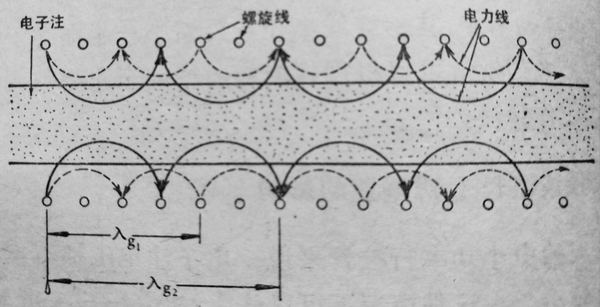
\includegraphics[width=0.65\linewidth]{figure/ch4-1}
	\caption{慢波波长改变时,高频场电力线形状变化示意图}
	\label{ch4-1}
\end{figure}

\begin{figure}[phtb]
	\centering
	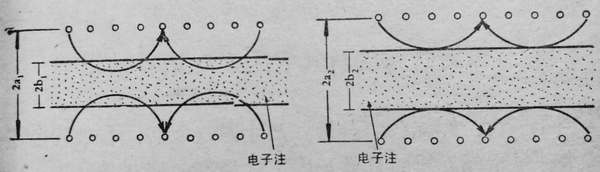
\includegraphics[width=0.65\linewidth]{figure/ch4-2}
	\caption{螺旋线直径增大后,进入电子注的电力线减少}
	\label{ch4-2}
\end{figure}

\begin{figure}[phtb]
	\centering
	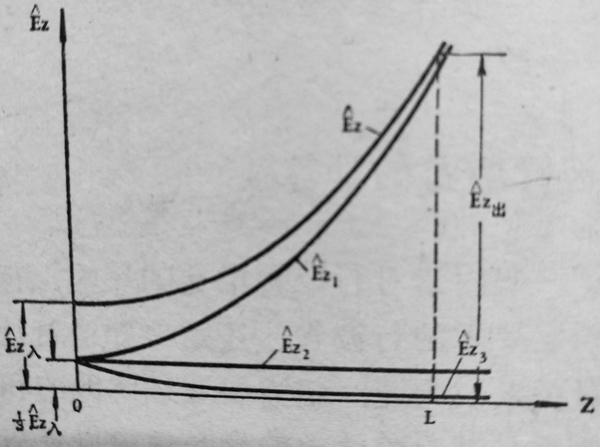
\includegraphics[width=0.65\linewidth]{figure/ch4-3}
	\caption{轴向高频电场沿$ Z $轴变化情况示意图}
	\label{ch4-3}
\end{figure}






